\documentclass[tikz, border=5pt]{standalone}
    \usepackage[utf8]{inputenc}
\usepackage[spanish]{babel}
\usepackage{tikz}
\usetikzlibrary{calc}
\usetikzlibrary{arrows}      
\usetikzlibrary{decorations.markings}
\usepackage{graphicx}
\DeclareGraphicsExtensions{.pdf,.png,.jpg}

\begin{document}
\begin{tikzpicture}{font=\Huge}
    \node at (0, 0) {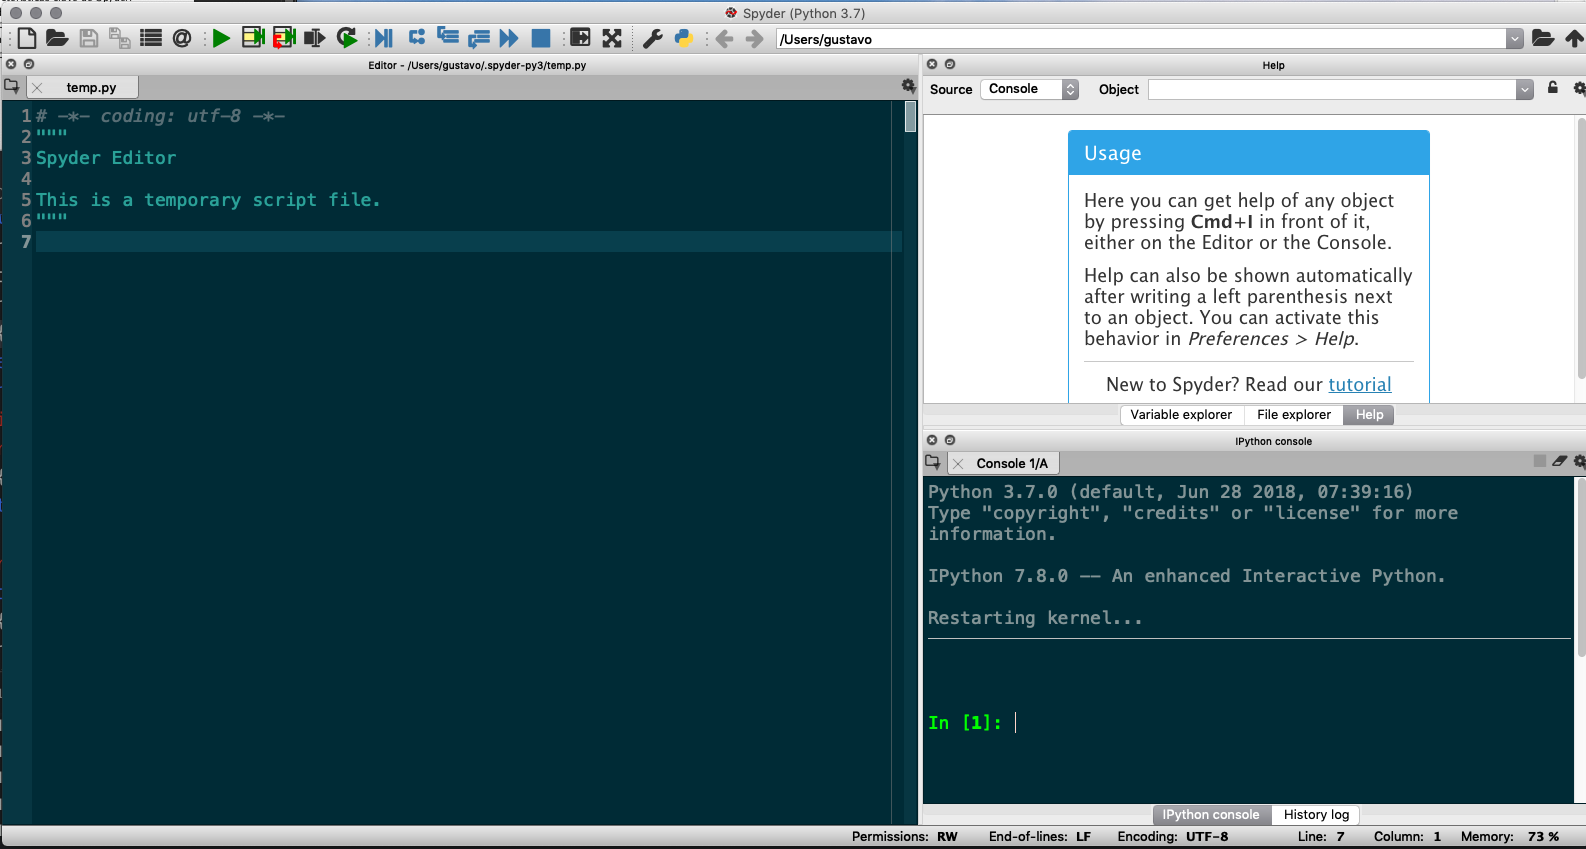
\includegraphics[scale=0.25]{spyder_02.png}};
    \draw [fill=yellow!50!white, opacity=0.3] (-7, -3.5) rectangle (1, 3);
    \node [text=white, scale=1.5] at (-3, 0) {Área del editor};
    \draw [fill=blue!50!white, opacity=0.3] (1.1, 0) rectangle (7, 3);
    \node [text=red, align=center] at (4, 2.5) {Área del explorador \\ y variables};
    \draw [fill=red!50!white, opacity=0.3] (1.1, -0.3) rectangle (7, -3.3);
    \node [text=white] at (4, -3) {Área de la terminal};
\end{tikzpicture}
\end{document}